\documentclass{article}
\usepackage{textcomp, gensymb}
\usepackage{utf8add}
\usepackage[most]{tcolorbox}
\usepackage{hyperref}
\usepackage{cleveref}
\usepackage{amsmath}
\usepackage{amssymb}
\usepackage{tcolorbox}
\usepackage{outlines}
\usepackage{enumitem}
\usepackage{graphics}
\usepackage{bbm}
% \usepackage{hhline}

\hypersetup{
    colorlinks,
    citecolor=black,
    filecolor=black,
    linkcolor=black,
    urlcolor=black
}
\DeclareMathOperator*{\argmax}{arg\,max}
\DeclareMathOperator*{\argmin}{arg\,min}

% \setenumerate[1]{label=\Roman*.}
% \setenumerate[2]{label=\Alph*.}
% \setenumerate[3]{label=\roman*.}
% \setenumerate[4]{label=\alph*.}

\title{CMPUT 428: 3D Modeling}
\author{Roderick Lan}
% \date{January 11, 2024}
\date{}

\usepackage{natbib}
\makeatletter
% \crefformat{tcb@cnt@Example}{example~#2#1#3}
% \Crefformat{tcb@cnt@Example}{Example~#2#1#3}
\makeatother
\newtcbtheorem[auto counter, number within = subsection]
{definition}{Definition}{%                                                        
  breakable,
  fonttitle = \bfseries,
  colframe = blue!75!black,
  colback = blue!10
}{def}

\makeatother
\newtcbtheorem[auto counter, number within = subsection]
{example}{Example}{%                                                        
  breakable,
  fonttitle = \bfseries,
  colframe = orange!75!black,
  colback = orange!10
}{ex}

\makeatother
\newtcbtheorem[auto counter, number within = subsection]
{expln}{Expln}{%                                                        
  breakable,
  fonttitle = \bfseries,
  colframe = red!75!black,
  colback = red!10
}{exp}

\makeatother
\newtcbtheorem[auto counter, number within = subsection]
{ovr}{Overview}{%                                                        
  breakable,
  fonttitle = \bfseries,
  colframe = blue!75!black,
  colback = blue!10!white!50
}{ovr}


\makeatother
\newtcbtheorem[auto counter, number within = subsection]
{refer}{Reference}{%                                                        
  breakable,
  fonttitle = \bfseries,
  colframe = red!75!black,
  colback = red!10
}{refer}
\begin{document}

\makeatother
\newtcbtheorem[auto counter, number within = subsection]
{thm}{Thm}{%                                                        
  breakable,
  fonttitle = \bfseries,
  colframe = orange!75!black,
  colback = orange!10
}{thm}

% \setcounter{section}{1}
\maketitle
\tableofcontents
\break
% \section*{Lecture 1}

\section{Lecture - Mar 12}
Lec09DynTextimpColl12\\[10pt]
Structure from Silhouette
\begin{list}{}{}
  \item Get cone ray from silhouette
\end{list}

\subsection{Incremental Free Space Carving}
Triangulate sparse point cloud: remove tetrahedrons/triangles + remake w/ points

\subsection{3D modeling system}
online, incremental handling of new info events
\\
works with sparse point clouds (good for vision/feature based methods)
\\
models coarse


\subsection{3 Tier Model}
Macro, Meso, Micro model
\\
refine geometry w/ coarse model as prior
\noindent
Multi Tiered Models:
\begin{outline}
  \1 Commonly:
    \2 2 Tiers: 3D geom and appearance (texture mapping)
    \2 Used in graphics applications, recovered from vision applications
  \1 3 Tier:
    \2 Macro - scene geometry (triangulation map)
    \2 Meso - fine scale geometric detail (displacement map)
    \3 Micro - fine scale geometry/reflectance (texture map)
  \1 Captured via sequential refinement
\end{outline}

\subsection{Multiscale Model}
Geometry alone doesnt solve modeling, need multiscale model
\\
Need
\begin{enumerate}
  \item Geometry
  \item Depth
  \item Dynamic Texture
\end{enumerate}
$\to$ Rendering
\\
Use image derivatives (know lighting changes, position of view, etc.) in forward way to render a diff. img (helps get photorealism)


\subsection{Capgui}
\subsubsection*{Step 1 - Calibration}
\subsubsection*{Step 2 - Segmentation}
Get rid of background
\subsubsection*{Step 3 - Shape From Silhouette}
8-60 imgs
\\
multiple views of same object $\to$ intersect \textbf{gneeralized cones} generated by each img
to build a volume (guaranteed to contain object)
\\
limiting smallest vol. obtainable in this way is known as the \textbf{visual hull} of the object


\subsubsection{SFS methods}
Voxel based (use voxel grid rep.)
\begin{list}{}{}
  \item inaccurate
  \item triangulate w/ marching cubes algo
\end{list}
Image ray based (use image rays)
\begin{list}{}{}
  \item accurate
\end{list}
Axis aligned (use rectlinear rays (instead of camera rays), mark 'cut' points of 
image rays)
\begin{list}{}{}
  \item moderately accurate
  \item fast
  \item marching intersections algo
  \item (mix of img ray and voxel based)
\end{list}

\subsubsection*{Step 4 - Phototextures + Texture Mapping}
For each triangle in model, establish corresponding region in the phototextures
\\
\textbf{Difficulties:}
\begin{outline}
  \1 Tedious to sepcify texture coords. for every triangle
  % \1 Acqui
\end{outline}

\subsubsection{Common Text. Coord. Mappings}
Orthogonal
\\
Cylindrical
\\
Spherical
\\
Perspective Projection
\\
Texture Chart (ie. text. split + flatten; cut object into pieces and map textures to each piece (piecwise planner))

\subsubsection{Advanced Texture Splitting and Mapping}
\textbf{Floating Planes} Method
\begin{outline}
  \1 split into dozen - several dozen perspective mappings
  \1 union of persp. planes accurately represent obj
\end{outline}
\noindent
\textbf{LCSM (Least Squares Conformal Mapping)}
\begin{outline}
  \1 least square (locally) preserve orthogonality
\end{outline}




\subsubsection*{Step 6 - Texture Basis Computation}


\noindent\rule{\textwidth}{0.1pt}

\subsection{Performance}
Can have many gb of texture memory
\\
Key issue: efficient memory access and processing
\begin{enumerate}
  \item Macro - conventional geom processing
  \item Meso - pixel shader; fixed code and variable data access
  \item Micro - Shader/Registration comb.; fixed code and fixed data access 
\end{enumerate}
% \subsection{Dyntex Theory}
\subsection{Meso Struct}
Depth with respect ot plane, doesnt work well with just one image (flat texture)
\subsubsection{Computing Meso}
Variational shape and reflectance
Per point cost func:
\[
  \mathbf{\phi (X,n)} = \sum_{i} h(\mathbf X, P_i)
  \|
  I_i (P_i(\mathbf X)) - R(\mathbf{X, n, L})
  \|
\]
$h$ $\to$ visibility + sampling
\\
$R$ $\to$ reflectance

\subsubsection{Rendering Meso}
% \begin{enumerate}
%   \item Sample d and ray at $N$ (\textasciitilde 15 pts)
% \end{enumerate}
$> 100$ fps for consumer GPU


\subsection{Micro Struct}
Spatial texture basis\\
Render temporally varying dynamic texture by modulating a linear basis
\\
Basis contains spatial derivs of img
\\
Rendered by linear blending (?)
\begin{list}{}{}
  \item fixed execution and data access pattern
  \item very fast implementation in graphics hardware
\end{list}
Can be done quickly in assembly (register extr.)

\subsubsection{Dynamic Textures}
3D geom and texture warp map b/w views and texture imgs
\\[5pt]
Diff texture img for each view;\\
A number of different misalignments 
\\[5pt]
Planar error - incorrect texture coords
\\
Out of plane error - object surface $\ne$ texture plane
\subsection{Spatial Basis Intro}
Moving sine wave can be modeled
\begin{flalign*}
  I (t) &= \sin (u + at) \\
  &=\sin(u)\cos(at) + \cos(u)\sin(at) \\
  &=\sin(u)y_1(t) + \cos(u)y_2(t)
\end{flalign*}
$u$ spatially fixed basis
\\[5pt]
Small image motion
\[
  I = I_0 + \frac{\partial I}{\partial u} \Delta u + \frac{\partial I}{\partial v}\Delta v
\]
Spatial fixed basis

\subsection{Linear basis for spatio-temporal variation}
On the obj./texture plane:
\begin{list}{}{}
  \item variation resulting from small warp perturbation
  \item Taylor expansion
  \begin{center}
    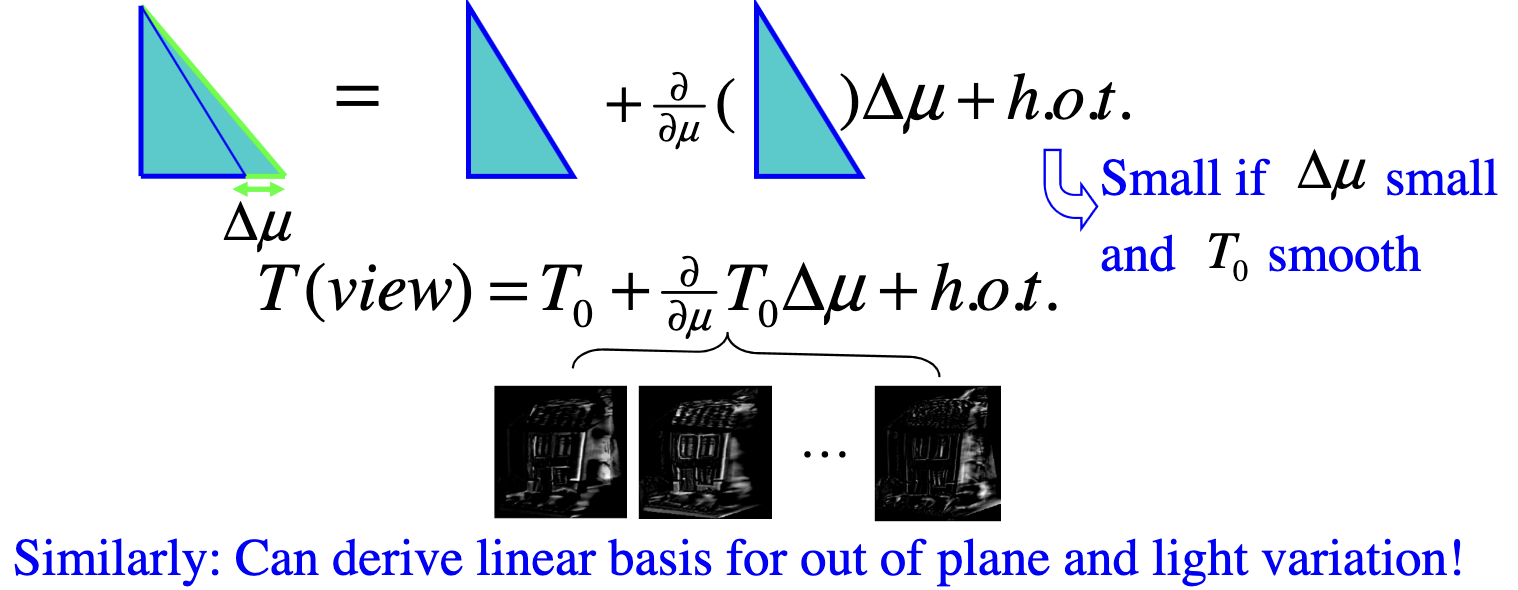
\includegraphics[width=.6\textwidth]{"imgs/taylor expansion mar12.png"}
  \end{center}
\end{list}

\subsection{Geometric spatial temporal variability}
Image 'warp'
\[
  T(\mathbf x) = I(W(\mathbf x ,\mu))
\]
Image variability caused by imperfect warp
\[
  \Delta T = I(W(\mathbf x, \mu + \Delta \mu)) - T_w
\]
First order approx.
\[
  \Delta T = I(W(\mathbf x, \mu)) + \nabla T \frac{\partial W}{\partial \mu} - T_w=
  \nabla T \frac{\partial W}{\partial \mu}
\]
Concrete examples: img plane; out of plane
\subsection{Variability due to a planar projective warp (homography)}
\subsection{Out of Plane Variability}
\subsection{Photometric Variation}
light changes how obj looks (?)
\\
dont need to raytrace


\subsection{Composite Variability}
composite texture intesity variability
\[
  \Delta \mathbf T = \Delta \mathbf T_s + \Delta \mathbf T_d + \Delta \mathbf T_l + \Delta \mathbf T_e
\]
planar + depth + light + res. err.
\\[5pt]
Can be modeled as sum of basis
\begin{flalign*}
  \Delta \mathbf T &= \mathbf{B_s y_s} + \mathbf{B_d y_d} + \mathbf{B_l y_l} + \Delta \mathbf(T_e)
  \\
  &= \mathbf{By + \Delta T_e}
\end{flalign*}

\subsection{How to Compute}
Slide 31 - 32 



\subsection{Dyntex}


\end{document}

